\documentclass{article}
%\usepackage[spanish,activeacute]{babel}
%\usepackage[english,activeacute]{babel}
%\usepackage[latin1]{inputenc}
\usepackage[utf8]{inputenc}
\usepackage[english]{babel}

\usepackage{amsmath,amsfonts,amssymb,amstext,amsthm,amscd}
\usepackage{hyperref}
\usepackage{latexsym}
\usepackage{graphicx}
%\usepackage{subfigure}
\usepackage{subfig}
%\linespread{1.6}
\usepackage{float}
\usepackage{dcolumn}% Align table columns on decimal point(esto lo saque del ejemplo de revtex4)
\usepackage{bm}% bold math(esto lo saque del ejemplo de revtex4)
\newcounter{itemR}
\usepackage{here} %recordar usar el comando[H] para las gráficas que es el comando here en lugar de [h!]
\usepackage{fancyhdr}
%\usepackage{sidecap}
%\usepackage[spanish,activeacute]{babel}
\usepackage{multirow}
\usepackage{multicol}
\usepackage{array}
\usepackage{enumitem}
%\usepackage{booktabs}% para hacer tablas profesionales con \toprule

% ------------------------------------------------------------------------------------------------------------------------------------------------------

\usepackage{fancyhdr}
\setlength{\headheight}{15.2pt}
\usepackage[paperwidth=8.5in, paperheight=11.0in, top=1.0in, bottom=1.0in, left=1.0in, right=1.0in]{geometry}

\pagestyle{fancyplain}
\fancyhead[LE,RO]{Práctica $\#$5}
\fancyhead[CE,CO]{}
\fancyhead[RE,LO]{P23-FIS1012-12}
\fancyfoot[LE,RO]{\thepage}
\fancyfoot[CE,CO]{Laboratorio de Física, UDLAP}
\fancyfoot[RE,LO]{}

% ------------------------------------------------------------------------------------------------------------------------------------------------------
% ------------------------------------------------------------------------------------------------------------------------------------------------------
% ------------------------------------------------------------------------------------------------------------------------------------------------------

\begin{document}

\fancypagestyle{plain}{
   	\renewcommand{\headrulewidth}{1pt}
   	\renewcommand{\footrulewidth}{1pt}
}

\renewcommand{\footrulewidth}{1pt}
\renewcommand{\tablename}{Tabla}
\renewcommand{\figurename}{Figura}

% ------------------------------------------------------------------------------------------------------------------------------------------------------
% ------------------------------------------------------------------------------------------------------------------------------------------------------
% ------------------------------------------------------------------------------------------------------------------------------------------------------

\title{Capacitores}
\author{\small{Luis Alberto Gil Bocanegra ID: 177410, Erick Gonzalez Parada ID: 178145}\\
 \small{Gartzen Aldecoa Barroso ID: 178034 .}\\		% ----- Varios autores separarlos por comas:  \small{Nombre(s) de (los) autor(es)\footnote{ID; correo@udlap.mx}, Nombre(s) de (los) autor(es)\footnote{ID; correo@udlap.mx}
	   \small{Depto. de Actuaría, Física y Matemáticas, Universidad de las Américas Puebla, Puebla, M\'exico 72810}}
\date{\small{\today}}

\maketitle

% ------------------------------------------------------------------------------------------------------------------------------------------------------
% ------------------------------------------------------------------------------------------------------------------------------------------------------
% ------------------------------------------------------------------------------------------------------------------------------------------------------

\begin{abstract}
	En esta práctica se observo los cambios de la capacitancia con respecto a los materiales 
	dieléctrico.
\\
\\
{\it Keywords:}  dieléctrico, capacitor 
\\
\\
\end{abstract}

% ------------------------------------------------------------------------------------------------------------------------------------------------------

\begin{multicols}{2}

\section{Desarrollo teórico}\label{Desarrollo Teorico}                              	% -------------------- Introducción
El objetivo de la práctica es determinar el comportamiento de la
capacitancia en función de la distancia y las
propiedades de los dieléctricos.
\cite{Quartux Enería}
La capacitancia es una propiedad fundamental en la teoría de circuitos eléctricos. Se define como la capacidad de un objeto o sistema para almacenar carga eléctrica. En el marco teórico de la capacitancia, se utiliza el concepto de condensadores, que son dispositivos diseñados específicamente para almacenar carga. La capacitancia (\(C\)) de un condensador se calcula como la relación entre la carga (\(Q\)) almacenada en el condensador y la diferencia de potencial (\(V\)) entre sus placas, es decir:

\[
C = \frac{Q}{V}
\]

Donde \(C\) se mide en faradios (F), \(Q\) en coulombs (C), y \(V\) en voltios (V). El marco teórico de la capacitancia es esencial para comprender cómo los condensadores interactúan en circuitos eléctricos, almacenando y liberando energía eléctrica según las leyes de la física electromagnética.

La ecuación \(C = \kappa C_{\text{aire}}\) se refiere a la capacitancia de un condensador, donde:

\begin{itemize}
    \item \(C\) es la capacitancia del condensador.
    \item \(\kappa\) es la constante dieléctrica del material entre las placas del condensador.
    \item \(C_{\text{aire}}\) es la capacitancia que tendría el condensador si el espacio entre las placas estuviera lleno de aire (un dieléctrico con constante dieléctrica igual a 1).
\end{itemize}

La constante dieléctrica (\(\kappa\)) representa la capacidad de un material para aumentar la capacitancia en comparación con el aire. Cuanto mayor sea \(\kappa\), mayor será la capacitancia en el mismo espacio entre las placas.

Además, la proporcionalidad entre la diferencia de potencial (\(\Delta V\)) y la carga (\(q\)) se expresa como \(|\Delta V| \propto |q|\). Esto significa que a medida que aumenta la carga en un condensador, la diferencia de potencial entre las placas también aumenta de manera proporcional.

La unidad de capacitancia es el faradio (\(1 \, \text{F}\)), que se define como \(1 \, \text{C} / 1 \, \text{V}\), lo que significa que un condensador tiene una capacitancia de 1 faradio si una carga de 1 coulomb produce una diferencia de potencial de 1 voltio entre sus placas.


\section{Desarrollo Experimental}\label{Desarrollo experimental}				% -------------------- Metodología 
%'
\subsection*{Lista de Materiales}
A continuación se presenta una lista de materiales:

\begin{enumerate}
    \item Capacitor físico variable
    \item Multímetro
    \item Vernier digital
    \item Dieléctricos
    \item 1 caja (24 piezas)
\end{enumerate}

Se conecto el multímetro de tal manera que depositara carga en el capacitor, se colocaron
diferentes materiales dieléctricos como acrílico de distintos grosores y cartón después se
extrajo la capacitancia detectada en el multímetro para empezar a ver la relación de capacitancia    
entre los dieléctricos, también se midió la distancia.
\\
 se realizó la graficación de la capacitancia en función de la distancia entre las placas,
 y se agregó una línea de tendencia a la gráfica resultante.
 Luego, se procedió a gráfica la capacitancia del condensador 
 frente a la capacitancia del dieléctrico, nuevamente incorporando una línea de tendencia a la gráfica.
\\
 Finalmente, utilizando la información obtenida de las gráficas anteriores,
  se llevó a cabo un análisis para determinar la constante dieléctrica 
(k) del material y, en última instancia, se identificó el tipo de material en base a esta constante.
 Estas acciones jugaron un papel crucial en la caracterización del material del condensador y en la comprensión
  de su comportamiento en función de la distancia y la capacitancia.
\end{multicols}
\section{Resultados y análisis}\label{Resultados}			% -------------------- Resultados
A continuación se presentan todas las gráficas de capacitancia vs distancia.

\begin{figure}[H]
	\centering	
	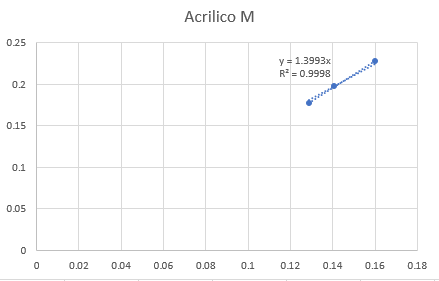
\includegraphics[scale=0.6]{../imgs/AcrilicoM.png}
	\caption{Acrílico mediano, capacitancia vs aire}
	\label{fig:1}
\end{figure}

\begin{figure}[H]
	\centering	
	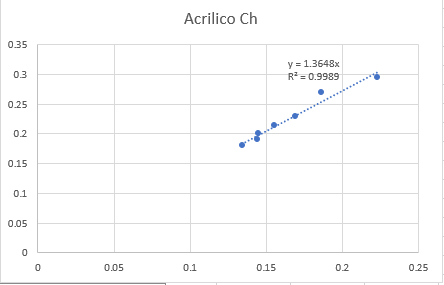
\includegraphics[scale=0.6]{../imgs/acrilicoch.png}
	\caption{Acrílico chico, capacitancia vs aire}
	\label{fig:2}
\end{figure}

\begin{figure}[H]
	\centering	
	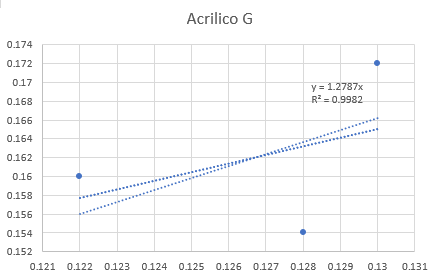
\includegraphics[scale=0.6]{../imgs/acrilicog.png}
	\caption{Acrílico grande, capacitancia vs aire}
	\label{fig:3}
\end{figure}

\begin{figure}[H]
	\centering	
	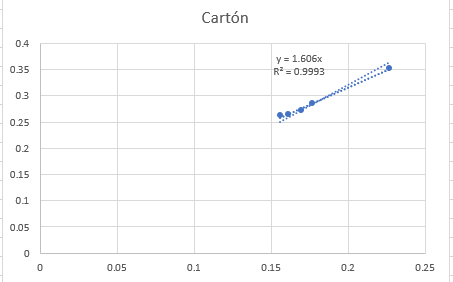
\includegraphics[scale=0.6]{../imgs/carton.png}
	\caption{cartón, capacitancia vs aire}
	\label{fig:4}
\end{figure}

\begin{figure}[H]
	\centering	
	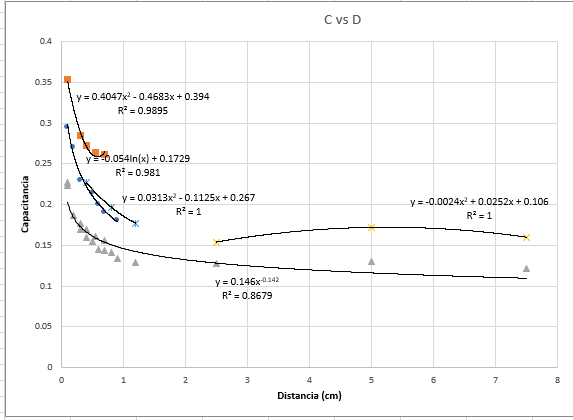
\includegraphics[scale=0.4]{../imgs/cvsd.png}
	\caption{todas las capacitancias vs distancia}
	\label{fig:5}
\end{figure}

Como se muestra en todas las figuras podemos apreciar como el potencial eléctrico es 
proporcional a la carga, esto debido a que un capacitor es mejor si podemos tener una mayor carga.
\\
Observamos también que en la figura \ref{fig:5} vemos que el aire en la mayoría de los casos   
es peor y que a mayor distancia menos capacitancia.
Podemos deducir el material por medio de kappa que en el caso de las gráficas es nuestro R.
\section{Conclusiones}\label{Conclusiones}				% -------------------- Conclusiones
Como equipo concluimos que el objetivo se cumplió ya que gracias a las gráficas siempre se puede concluir 
un comportamiento entre los elementos y como se menciono podemos deducir el tipo de material con respecto 
a la constante dieléctrica.

\begin{thebibliography}{9}						% -------------------- Bibliografía
	\bibitem{Quartux Enería}
	¿Qué es un capacitor eléctrico? | Quartux Energía | Quartux. (s. f.). https://www.quartux.com/blog/que-es-un-capacitor-o-condensador-electrico
	\bibitem{Serway}
	Serway, R. A., $\&$ Jewett, J. W. (2008). Física para ciencias e ingeniería. (7.a
ed., Vol. 1). CENGAGE Learning.

\bibitem{Pérez}
	Newton, I. (1687). Philosophiæ Naturalis Principia Mathematica [Mathematical Principles of Natural Philosophy]. Londini: Jussu Societatis Regiæ ac Typis Josephi Streater.

\end{thebibliography}
\end{document}	